\section{Introducción}

\begin{subsection}{FuDePAN}
 
\begin{frame}\frametitle{\small{Fundación para el Desarrollo de la Programación en Ácidos Nucleicos}}
  \fude\ es una ONG (organización no gubernamental) concebida para fomentar el desarrollo de técnicas y tecnologías
  para la Programación en \'Acidos Nucleicos, al servicio de la salud humana y animal.\\[0.2cm]
  \pause
  \begin{itemize}
    \item Fundada en 2006.
    \item Bioinformática ingenieril.
    \item I+D.
    \item Colaboran
        \begin{itemize}
            \item Estudiantes: Voluntarios y tesistas
            \item Profesionales: Ámbito industrial y académico.
        \end{itemize}

    \item Todo lo desarrollado por la fundación se encuentra bajo GPLv3.
  \end{itemize}
\end{frame}

\begin{frame}\frametitle{\small{Fundación para el Desarrollo de la Programación en Ácidos Nucleicos}}
    \large{\textbf{Pilares}}
    \begin{center}
        
\includegraphics[scale=0.30]{images/fudesuma.png}
    \end{center}
    \pause
    \begin{block}{Naturaleza de los problemas}
        \begin{itemize}
            \item Corren mucho tiempo
            \item Alta performance
            \item Resultados impactan en nuevos problemas y personas.
        \end{itemize}
    \end{block}
\end{frame}

\end{subsection}

\begin{subsection}{Motivación}

\begin{frame}\frametitle{Motivación}
    La fundación necesitaba una librería que facilitara el desarrollo de un gran número de proyectos bioinformáticos que usan a la
    recursión como mecanismo fundamental. Esta abstracción abarca la familia de problemas que cumplen las siguientes condiciones:\\[0.2cm]
    \begin{itemize}
        \item   la solución se adapte a un modelo recursivo (principalmente para aquellas soluciones con definición inherentemente
                recursiva),
        \item   haya independencia de datos entre los nodos del árbol de recursión de la solución.
    \end{itemize}

    \pause
    \begin{block}{}
        Debido a que la mayoría de estos problemas requieren un alto nivel de cómputo, se eligió implementar este trabajo como una
        nueva capa sobre el framework de aplicaciones distribuidas \fud.
    \end{block}
\end{frame}

\end{subsection}

\begin{subsection}{FuD}

\begin{frame}\frametitle{FuD}

    \begin{block}{Definición}
        \fud\ (\textbf{F}uDePAN \textbf{U}biquitous \textbf{D}istribution) Es un framework para automatizar la distribución de aplicaciones
        computacionales a través de disposiciones heterogéneas y dinámicas de nodos de procesamiento.
    \end{block}

    \pause
    \textbf{Características}
    \begin{itemize}
%         \item Permite implementar de manera sencilla soluciones informáticas que hagan uso de técnicas distribuidas de programación.
        \item Facilidad para implementar soluciones informáticas paralelas.
        \item Flexibilidad para desarrollar cualquier problema computacional.
%         \item Independiente de los recursos que se dispondrán eventualmente para llevar a cabo el cómputo.
        \item Independencia de recursos.
        \item Abstrae del medio de distribución (BOINC, clusters, etc.)
        \item Arquitectura \textit{Master-Worker} con paralelismo de datos
        \item Extensible, permitiendo acotación de familias de problemas
            \begin{itemize}
                \item \textbf{RecAbs}
                \item \textbf{CombEng}
            \end{itemize}
    \end{itemize}
    
\end{frame}

\begin{frame}\frametitle{Ensures}

    \begin{itemize}
        \item Que la aplicaci\'on implementada tiene el potencial de ejecutarse paralelamente.
    %      \pause
        \item Que la aplicaci\'on explotar\'a los recursos que se pongan a su disposici\'on.
    %      \pause
        \item El uso del framework no generar\'a p\'erdidas de performance considerables.
    %      \pause
        \item Los datos intercambiados entre aplicaciones cliente y servidor no llevar\'an una carga adicional significativa sobre los datos
        necesarios para la aplicaci\'on.
        \end{itemize}
    \end{frame}

\begin{frame}\frametitle{Arquitectura}
     \begin{center}
        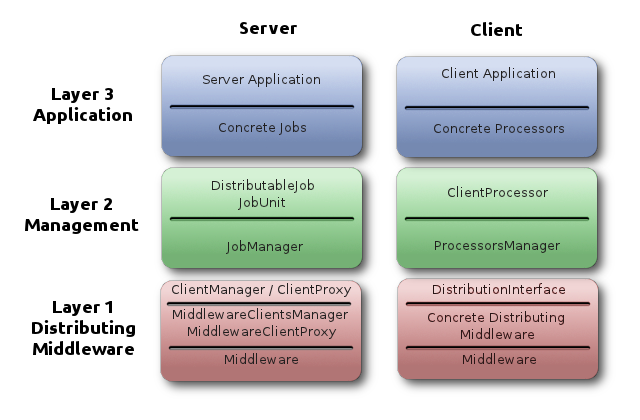
\includegraphics[scale=.45]{images/FuD-AbstractLayers.png}
      \end{center}
\end{frame}

\end{subsection}

% \begin{subsection}{Marco Teórico}
%     \begin{frame}
% 
%     \end{frame}
% \end{subsection}
